\chapter{Resultaten en evaluatie}
\label{ch:resultaten-evaluatie}

In dit hoofdstuk worden de resultaten van de verschillende getrainde modellen met elkaar vergeleken. De focus ligt daarbij op drie grote categorieën van trainingsstrategieën: supervised learning, \gls{ssl} (hier vertegenwoordigd door FixMatch) en \gls{self-sl} (hier via \gls{byol}). Door deze methodes systematisch te vergelijken, kan worden nagegaan hoe goed elk type model presteert bij een gelimiteerde hoeveelheid gelabelde data, en welke strategie het meest efficiënt is in het benutten van die data. \\

\section{Resultatenvergelijking: supervised vs SSL vs Self-SL}

Supervised learning vormt de klassieke aanpak waarbij modellen uitsluitend trainen op volledig gelabelde datasets. In dit onderzoek werden modellen getraind met verschillende percentages gelabelde data: 1\%, 5\%, 10\%, 50\% en 100\%. Deze variatie biedt inzicht in hoe sterk de performantie van een model afhankelijk is van de hoeveelheid supervisie, en dient als referentiepunt voor de andere methodes. \\

De \gls{ssl} aanpak via FixMatch combineert een kleine hoeveelheid gelabelde data met een grotere hoeveelheid ongelabelde data, waarbij het model zelf pseudo-labels genereert op basis van zijn voorspellingen. Deze pseudo-labels worden vervolgens gebruikt om het model verder te trainen. FixMatch is specifiek ontworpen om sterke resultaten te behalen met een beperkte gelabelde subset, door slim gebruik te maken van augmentaties en consistentie tussen voorspellingen. \\

\Gls{self-sl}, in dit geval via \gls{byol}, leert representaties zonder enige labelinformatie, door middel van contrastieve technieken waarbij het model leert om verschillende weergaven van hetzelfde beeld te associëren. Deze representaties worden vervolgens gebruikt om een objectdetector te trainen met beperkte supervisie. \Gls{self-sl} is vooral interessant omwille van zijn label-onafhankelijkheid in de pretrainingsfase. \\

De vergelijking tussen deze methodes biedt niet enkel inzicht in de accuraatheid en generalisatiecapaciteit van de modellen, maar legt ook bloot hoe efficiënt elk type benadering omgaat met beperkte annotatie. Daarbij wordt zowel een kwantitatieve (via \gls{map}) als kwalitatieve analyse uitgevoerd, om de sterktes en beperkingen van elke methode in de praktijk te evalueren.

\section{Kwantitatieve analyse}

De prestaties van de verschillende modellen en trainingsstrategieën zijn overzichtelijk samengevat in Tabel \ref{tab:map-results}. Deze tabel toont de \gls{map} scores voor Faster \gls{rcnn} bij verschillende percentages gelabelde data, alsook de resultaten van \gls{ssl} FixMatch en \gls{self-sl} \gls{byol} modellen getraind op respectievelijk 5\% en 10\% gelabelde data.

\begin{table}[H]
    \centering
    \begin{tabular}{ll}
        \toprule
        \textbf{Model en Gelabeld Percentage} & \textbf{mAP} \\
        \midrule
        Faster R-CNN 1\%                 & 0.2799 \\
        Faster R-CNN 5\%                 & 0.5298 \\
        Faster R-CNN 5\% + BYOL          & 0.6452 \\
        Faster R-CNN 10\%                & 0.6152 \\
        Faster R-CNN 10\% + BYOL         & 0.7230 \\
        Faster R-CNN 50\%                & 0.7847 \\
        Faster R-CNN 100\%               & 0.7717 \\
        FixMatch 5\%                    & 0.6649 \\
        FixMatch 10\%                   & 0.6828 \\
        \bottomrule
    \end{tabular}
    \caption[Overzicht van mAP-score van verschillende modellen.]{\label{tab:map-results}Overzicht van \gls{map}-resultaten voor verschillende modellen en gelabelde datavolumes.}
\end{table}

De evaluatie van de verschillende modellen en trainingsstrategieën laat duidelijke verschillen zien in prestaties gemeten aan de hand van de \gls{map}. Het baseline Faster \gls{rcnn} model, getraind op de volledige dataset (100\% gelabelde data), behaalt een \gls{map} van 0.7717, wat een solide uitgangspunt vormt voor vergelijking met modellen die minder gelabelde data gebruiken of \gls{ssl} en \gls{self-sl} technieken toepassen. \\

Wanneer de hoeveelheid gelabelde data wordt teruggebracht, daalt de prestaties van het supervised Faster \gls{rcnn} model significant. Bij 50\% gelabelde data stijgt de \gls{map} zelfs licht tot 0.7847, mogelijk door toeval of lichte verschillen in splitsing, maar bij verdere reductie naar 10\%, 5\% en 1\% zakt de \gls{map} respectievelijk naar 0.6152, 0.5298 en 0.2799. Dit bevestigt het belang van voldoende gelabelde data voor goede prestaties in traditionele supervised learning. \\

Figuur \ref{fig:map_different_splits} visualiseert deze trend duidelijk. Hierin is zichtbaar dat de performantie van het supervised model exponentieel afneemt naarmate de hoeveelheid gelabelde data wordt teruggeschroefd, wat de uitdaging benadrukt van voldoende annotations in sonardatasets.

\begin{figure}[H]
    \centering
    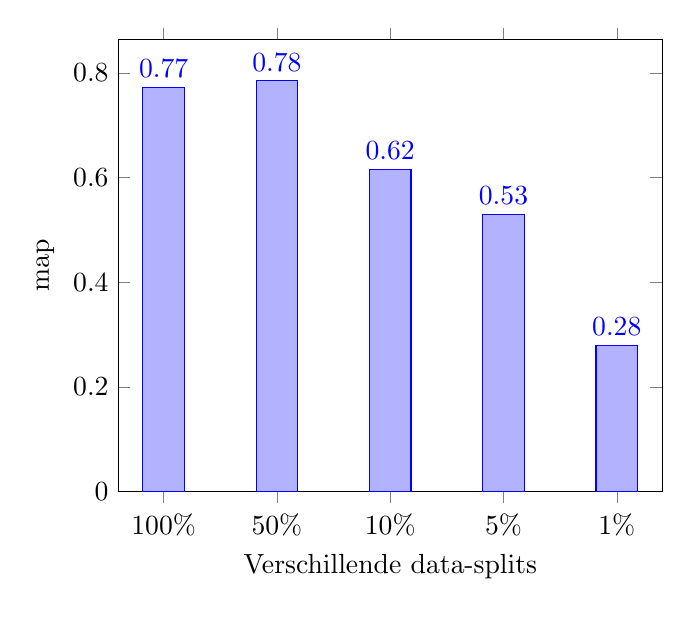
\begin{tikzpicture}
        \begin{axis}[
            ybar,
            width=0.7\textwidth,
            symbolic x coords={100\%, 50\%, 10\%, 5\%, 1\%},
            xtick=data,
            ymin=0,
            bar width=15pt,
            xlabel={Verschillende data-splits},
            ylabel={\gls{map}},
            nodes near coords,
            ]
            \addplot coordinates {(100\%,0.7717) (50\%,0.7847) (10\%,0.6152) (5\%,0.5298) (1\%,0.2799)};
        \end{axis}
    \end{tikzpicture}
    \caption[mAP voor Faster R-CNN met verschillende data-splits.]{\label{fig:map_different_splits}Overzicht van de \gls{map} voor de supervised Faster \gls{rcnn} modellen getraind op de verschillende data-splits.}
\end{figure}

De toepassing van \gls{self-sl} pretraining via \gls{byol}, gevolgd door fine-tuning met beperkte gelabelde data, laat een merkbare verbetering zien ten opzichte van het pure supervised model bij lage data-volumes. Figuur \ref{fig:map_performance_research_models} toont deze vergelijking van \gls{map}-scores. Zo verbetert de \gls{map} bij 5\% gelabelde data van 0.5298 (Faster \gls{rcnn}) naar 0.6452 (Faster \gls{rcnn} + \gls{byol}), en bij 10\% gelabelde data van 0.6152 naar 0.7230. Dit suggereert dat \gls{self-sl} pretraining effectief representaties leert die waardevol zijn voor downstream objectdetectie, waardoor het model minder afhankelijk wordt van grote hoeveelheden gelabelde data. \\

FixMatch, als \gls{ssl} methode, toont eveneens verbetering boven de pure supervised baseline bij 5\% en 10\% gelabelde data, met \gls{map}-waarden van respectievelijk 0.6649 en 0.6828. Hoewel FixMatch op 10\% iets onder het \gls{byol}-gefine-tunede model blijft, overtreft het de baseline aanzienlijk, wat de potentie van \gls{ssl} in dit domein onderstreept.

\begin{figure}[H]
    \centering
    \begin{tikzpicture}
        \begin{axis}[
            ybar,
            bar width=15pt,
            width=0.8\textwidth,
            enlargelimits=0.5,
            ybar=10pt,
            legend style={at={(0.5,-0.15)}, anchor=north,legend columns=-1},
            xlabel={Verschillende data-splits},
            ylabel={\gls{map}},
            ymax=0.7,
            symbolic x coords={10\%, 5\%},
            xtick=data,
            nodes near coords,
            nodes near coords align={vertical},
            ]
            \addplot coordinates {(10\%,0.6152) (5\%,0.5298)};
            \addplot coordinates {(10\%,0.6828) (5\%,0.6649)};
            \addplot coordinates {(10\%,0.7230) (5\%,0.6452)};
            \legend{Faster \acrshort{rcnn} baseline, FixMatch, \acrshort{byol}}
        \end{axis}
    \end{tikzpicture}
    \caption[Vergelijking van mAP tussen semi- en self-supervised modellen.]{\label{fig:map_performance_research_models}Overzicht van de \gls{map} voor het supervised Faster \gls{rcnn} model, het \gls{ssl} FixMatch model en het \gls{self-sl} \gls{byol} model, getraind op 10\% en 5\% data-splits.}
\end{figure}

Deze resultaten impliceren dat de combinatie van representatieleren via \gls{self-sl} pretraining of \gls{ssl} label-augmentatie het model minder afhankelijk maakt van grote hoeveelheden gelabelde data, wat cruciaal is voor kostbare domeinen als sonardata-analyse. De relatief kleine verschillen tussen FixMatch en \gls{byol} kunnen wijzen op verschillende sterke kanten van \gls{ssl} versus \gls{self-sl} methoden, afhankelijk van de dataset en de implementatie. \\

Daarnaast blijkt dat bij grotere hoeveelheden gelabelde data (50\% en 100\%) het pure supervised model nog steeds het beste scoort, hoewel de winst bij 100\% ten opzichte van 50\% beperkt is. Dit kan een indicatie zijn van een verzadigingseffect waarbij extra gelabelde data slechts marginale verbeteringen opleveren. Het \gls{ssl} en \gls{self-sl} trainen zijn dan minder noodzakelijk, maar kunnen nog steeds nuttig zijn om trainingskosten en annotatielast te reduceren.

\section{Kwalitatieve analyse}

Op basis van de visuele inspectie van de modelvoorspellingen biedt de kwalitatieve analyse waardevolle inzichten in het gedrag en de betrouwbaarheid van de verschillende detectiemodellen. De analyse is gebaseerd op twee figuren: één die de prestaties van de supervised modellen toont, en een tweede die de prestaties van de onderzochte \gls{ssl} en \gls{self-sl} modellen (FixMatch en \gls{byol}) vergelijkt met de ground truth.

\begin{figure}[H]
    \centering
    \begin{subfigure}{.2\textwidth}
        \centering
        \captionsetup{justification=centering}
        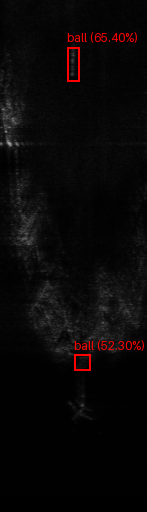
\includegraphics[width=0.9\linewidth]{251_faster_rcnn_1pct.png}
        \caption[Voorspelling Faster R-CNN 1\%]{1\%}
    \end{subfigure}%
    \begin{subfigure}{.2\textwidth}
        \centering
        \captionsetup{justification=centering}
        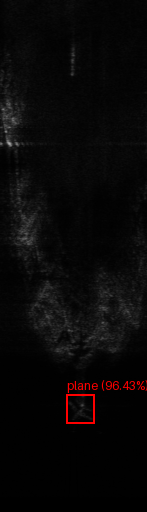
\includegraphics[width=0.9\linewidth]{251_faster_rcnn_5pct.png}
        \caption[Voorspelling Faster R-CNN 5\%]{5\%}
    \end{subfigure}%
    \begin{subfigure}{.2\textwidth}
        \centering
        \captionsetup{justification=centering}
        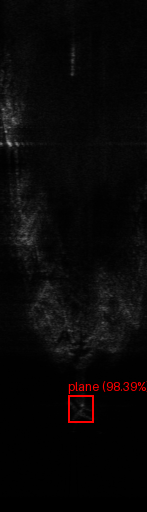
\includegraphics[width=0.9\linewidth]{251_faster_rcnn_10pct.png}
        \caption[Voorspelling Faster R-CNN 5\%]{5\%}
    \end{subfigure}%
    \begin{subfigure}{.2\textwidth}
        \centering
        \captionsetup{justification=centering}
        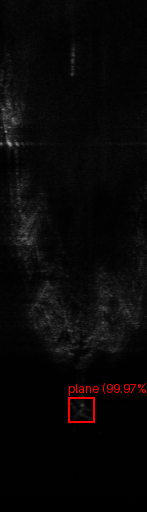
\includegraphics[width=0.9\linewidth]{251_faster_rcnn_50pct.png}
        \caption[Voorspelling Faster R-CNN 50\%]{50\%}
    \end{subfigure}%
    \begin{subfigure}{.2\textwidth}
        \centering
        \captionsetup{justification=centering}
        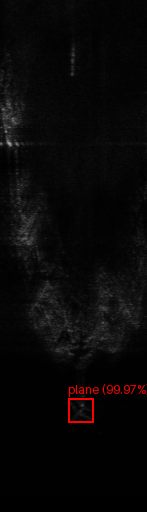
\includegraphics[width=0.9\linewidth]{251_faster_rcnn_100pct.png}
        \caption[Voorspelling Faster R-CNN 100\%]{100\%}
    \end{subfigure}%
    \caption[Voorspellingen door supervised modellen.]{Voorspellingen op afbeelding \texttt{00251} van de \texttt{UATD\_Test\_1}-dataset door Faster \gls{rcnn} getraind op verschillende subsets.}
\end{figure}

In de figuur met alle supervised modellen valt op dat de prestaties van de meeste modellen relatief sterk zijn, zelfs bij beperkte hoeveelheden gelabelde data. De detectie-outputs van de modellen getraind op 5\%, 10\%, 50\% en 100\% gelabelde data tonen telkens correcte identificaties van de objecten, met nauwkeurig geplaatste \glspl{bounding_box} en hoge \glspl{confidence_score}. Enkel het model getraind met slechts 1\% gelabelde data wijkt opvallend af. Dit model genereert foutieve voorspellingen, herkent objecten die niet aanwezig zijn, en doet dit bovendien met hoge \glspl{confidence_score}. Ook worden aanwezige objecten fout geclassificeerd. Deze bevinding bevestigt dat bij een te beperkte hoeveelheid gelabelde data het supervised model niet in staat is robuuste representaties te leren, wat leidt tot onbetrouwbare detectie.

\begin{figure}[H]
    \centering
    \begin{subfigure}{.2\textwidth}
        \centering
        \captionsetup{justification=centering}
        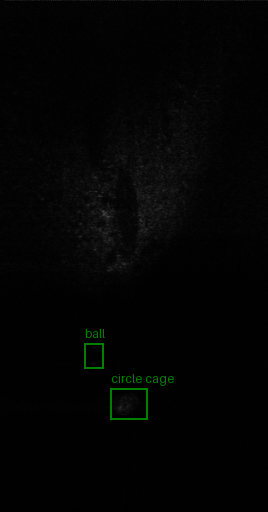
\includegraphics[width=0.9\linewidth]{1_gt.png}
        \caption[Ground truth]{Ground truth}
        \label{fig:ground_truth_}
    \end{subfigure}%
    \begin{subfigure}{.2\textwidth}
        \centering
        \captionsetup{justification=centering}
        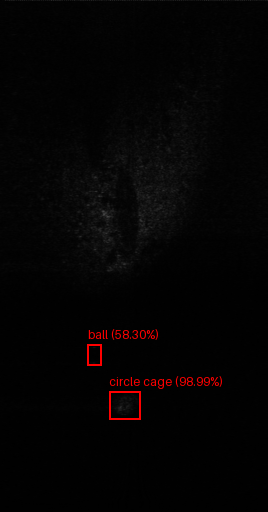
\includegraphics[width=0.9\linewidth]{1_fixmatch_10pct.png}
        \caption[Voorspelling FixMatch 10\%]{FixMatch 10\%}
        \label{fig:faster_rcnn_5_prediction}
    \end{subfigure}%
    \begin{subfigure}{.2\textwidth}
        \centering
        \captionsetup{justification=centering}
        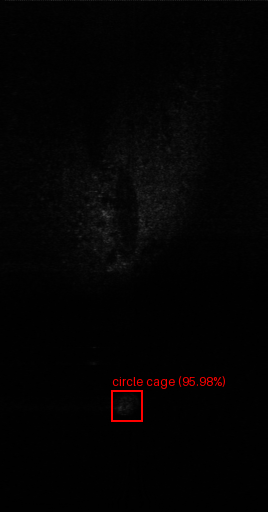
\includegraphics[width=0.9\linewidth]{1_fixmatch_5pct.png}
        \caption[Voorspelling FixMatch 5\%]{FixMatch 5\%}
        \label{fig:faster_rcnn_10_prediction}
    \end{subfigure}%
    \begin{subfigure}{.2\textwidth}
        \centering
        \captionsetup{justification=centering}
        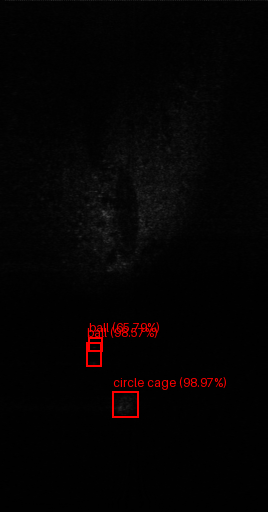
\includegraphics[width=0.9\linewidth]{1_faster_rcnn_10_byol.png}
        \caption[Voorspelling BYOL 10\%]{BYOL 10\%}
        \label{fig:faster_rcnn_50_prediction}
    \end{subfigure}%
    \begin{subfigure}{.2\textwidth}
        \centering
        \captionsetup{justification=centering}
        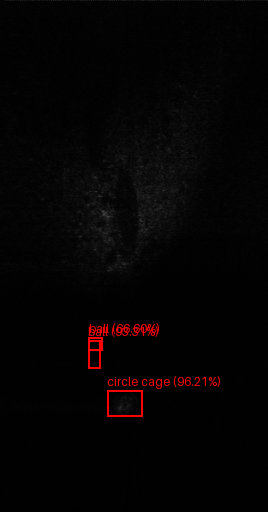
\includegraphics[width=0.9\linewidth]{1_faster_rcnn_5_byol.png}
        \caption[Voorspelling BYOL 5\%]{BYOL 5\%}
    \end{subfigure}%
    \caption[Voorspellingen door semi- en self-supervised modellen.]{Voorspellingen op afbeelding \texttt{00001} van de \texttt{UATD\_Test\_1}-dataset door FixMatch en Faster \gls{rcnn} + \gls{byol} getraind op verschillende subsets.}
    \label{fig:supervised_predictions}
\end{figure}

In de tweede figuur, waarin de voorspellingen van FixMatch en \gls{byol} vergeleken worden met de ground truth, komen enkele opvallende verschillen naar voren. Het FixMatch-model getraind met 10\% gelabelde data voorspelt alle objecten correct, maar doet dit met relatief lage \glspl{confidence_score} voor bepaalde objecten. Dit suggereert dat het model wel degelijk leert om relevante objectkenmerken te herkennen, maar minder zeker is van zijn voorspellingen -- mogelijk door de beperkte kwaliteit van de pseudo-labels tijdens het trainingsproces. Bij het FixMatch-model getraind met slechts 5\% gelabelde data ontbreekt één object volledig in de voorspellingen. Dit wijst op een verhoogde fragiliteit van het model bij nog beperktere labeling, wat impliceert dat de hoeveelheid gelabelde data bij FixMatch sterk correleert met de volledigheid van de voorspellingen. \\

De \gls{byol}-gebaseerde modellen vertonen een ander gedragspatroon. Zowel bij 5\% als bij 10\% gelabelde data worden alle objecten correct herkend en geclassificeerd. Dit bevestigt dat de representaties die via \gls{byol} geleerd worden, effectief zijn in het ondersteunen van objectdetectie bij gelimiteerde data. Echter, er worden opvallend veel \glspl{bounding_box} over elkaar heen voorspeld. Dit fenomeen duidt mogelijk op een tekort aan post-processing, met name het ontbreken of incorrect toepassen van \gls{nms}. Hoewel de onderliggende herkenning goed is, leidt dit gedrag tot redundante output die de interpretatie bemoeilijkt en de precisie negatief kan beïnvloeden.

\begin{figure}[H]
    \centering
    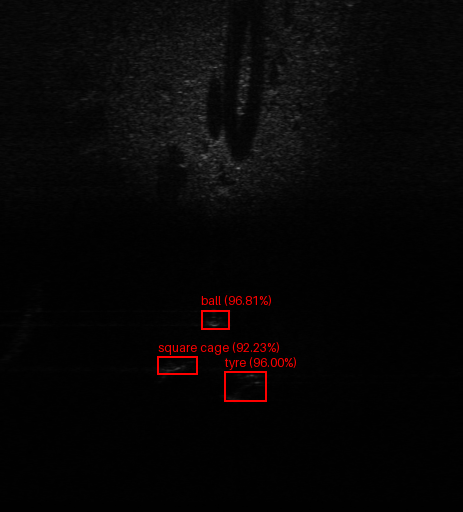
\includegraphics[width=0.7\textwidth]{8_faster_rcnn_5_byol.png}
    \caption[Correcte voorspellingen van BYOL 5\%]{\label{fig:faster_rcnn_correct}Correcte voorspellingen van Faster \gls{rcnn} 5\% + BYOL (afbeelding \texttt{00008} van de \texttt{UATD\_Test\_1}-dataset)}
\end{figure}

De kwalitatieve analyse bevestigt dat het gebruik van \gls{ssl} en \gls{self-sl} strategieën zinvol is bij gelimiteerde labeling. FixMatch lijkt gevoeliger voor labelhoeveelheid dan \gls{byol}, terwijl \gls{byol} robuuste detecties levert, maar extra optimalisatie vereist op het niveau van outputfiltering. De vergelijking met de supervised modellen toont aan dat vanaf 5\% gelabelde data al vrij betrouwbare prestaties gehaald worden, maar dat de meer geavanceerde pretrainingstrategieën een duidelijke meerwaarde kunnen bieden voor nauwkeurigheid en consistentie -- mits ze correct worden afgestemd.